\subsection{数据预处理与语义分割模块}
\par 该模块利用\texttt{Frame}类对每一帧图像进行统一管理,包括RGB图像、深度图像以及语义分割图像,组件图如图\ref{fig:component3}所示。

\par 当新一帧的数据通过数据采集模块获取后,首先对RGB图像和深度图像进行对齐。对齐的过程是
通过调用\texttt{AlignImage}实现的,它使用Intel RealSense相机内参以及RGB图像和深度图像的位姿矩阵
进行校准,从而确保了在后续的三维重建过程中,RGB像素点和对应深度像素点的时间戳是相同的。

\begin{figure}[htbp]
	\centering
	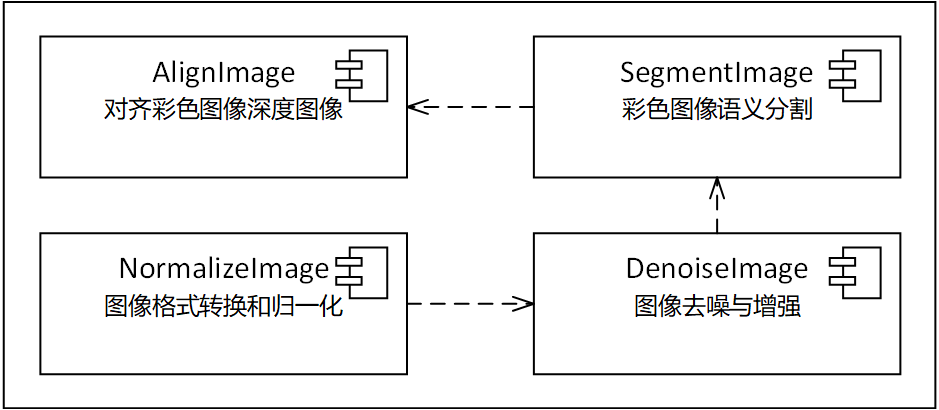
\includegraphics[width=0.7\textwidth]{figures/uml/component3.png}
	\caption{数据预处理与语义分割模块组件图}
	\label{fig:component3}
\end{figure}

\par 接着,系统将对RGB图像进行语义分割。这一步由\texttt{SegmentImage}完成,该函数会加载预训练的
“kMaX-DeepLab with ConvNeXt-large backbone with output stride 32” SavedModel模型进行推理,
为每个像素赋予一个类别标签。有了这些标签,系统就可以根据这些信息提高后续三维重建的精度和准确性。

% \begin{algorithm}[htb]
% 	\SetAlgoLined
% 	\KwData{RGB图像 rgb\_image, 模型路径 model\_path}
% 	\KwResult{语义分割图像 segmented\_image}
% 	% $\textit{session} \gets \text{TensorFlow.NewSession()}$\hspace{0.5cm}\tcp{创建一个新的TensorFlow会话}

% 	\tcp{创建一个新的TensorFlow会话}
% 	$\textit{session} \gets \text{TensorFlow.NewSession()}$\;

% 	\tcp{加载给定路径的模型}
% 	$\textit{graph\_def} \gets \text{TensorFlow.LoadModel}(\textit{model\_path})$\;

% 	\tcp{在会话中创建模型的图定义}
% 	$\textit{session.Create}(\textit{graph\_def})$\;

% 	\tcp{从RGB图像创建一个张量}
% 	$\textit{image\_tensor} \gets \text{CreateTensorFromImage}(\textit{rgb\_image})$\;

% 	\tcp{在会话中运行图像张量并获取输出}
% 	$\textit{outputs} \gets \text{session.Run}(\textit{image\_tensor})$\;

% 	\tcp{将输出结果转换为Mat类型的分割图像}
% 	$\textit{segmented\_image} \gets \text{ConvertOutputToMat}(\textit{outputs})$\;

% 	\caption{SegmentImage}
% 	\label{algo:SegmentImage}
% \end{algorithm}

\par 对图像进行语义分割之后,需要进行去噪与增强。\texttt{DenoiseImage}调用OpenCV的中值滤波函数接口 \texttt{cv::medianBlur}
和高斯滤波函数接口 \texttt{cv::GaussianBlur},去除图像中的脉冲噪声和高斯噪声。然后根据相机的视场、测量范围和深度信息,对图像进行裁剪,去除图像中的无效区域。接着,将RGB图像和语义分割图像缩放至$1296 \times 968$,将深度图像缩放至$640 \times 480$。

\begin{algorithm}[htbp]
	\SetAlgoLined
	\KwData{原始图像数据 src, 像素数组 des, 图像类型 type, 每行字节数 step}
	\KwResult{归一化图像数据}
	用块和线程索引初始化整数变量 $c$, $r$, $channel$, $w$, $h$\;
	\If{当前图像为RGB图像}{
		计算目标索引 $i = (r * w + c) * 3 + channel$\;
		使用 $v = int(src[r * step + c * 3 + channel])$ 从图像中获取像素值\;
		使用 $v = v / 255.0f$ 归一化值\;
		使用 $des[i] = v$ 将像素值赋给目标数组\;
	}
	\ElseIf{当前图像为深度图像}{
		初始化ushort变量 $depth\_us = 0$\;
		用 $depth\_us = depth\_us | src[r * step + c * 2 + 1]$ 更新 $depth\_us$\;
		改变字节序列 $depth\_us = depth\_us << 8$\;
		用 $depth\_us = depth\_us | src[r * step + c * 2]$ 更新 $depth\_us$\;
		使用 $depth\_val = (float)(depth\_us) / 1000.0f$ 归一化深度值\;
		如果深度值大于 6.0f,则设为 0.0f\;
		使用 $des[r * w + c] = depth\_val$ 将深度值赋给目标数组\;
	}
	\Else{
		计算目标索引 $i = (r * w + c) * 3 + channel$\;
		使用 $v = int(src[r * step + c * 3 + channel])$ 从图像中获取像素值\;
		如果通道是 2,使用 $v = v / 255.0f$ 归一化值\;
		使用 $des[i] = v$ 将值赋给目标数组\;
	}
	\caption{NormalizeImage}
	\label{algo:NormalizeImage}
\end{algorithm}

\par 最后,进行图像的格式转换和数值归一化。通过调用CUDA环境下运行的一个\texttt{\_\_global\_\_}函数
\texttt{NormalizeImage}实现,伪代码如算法\ref{algo:NormalizeImage}所示。输入参数中,\texttt{src}是原始图像数据,\texttt{des}是存放输出结果的像素数组,\texttt{type}用
于区分图像类型,\texttt{step}是图像中每行的字节数。该函数在CUDA内核中执行,利用
并行计算加速图像处理过程。该函数将图像的格式转换成系统规定的格式,并将每个像素的值归一化,
使得它们在0到1之间:

\par 首先,函数根据CUDA线程模型中的\texttt{blockIdx}和\texttt{threadIdx}来计算在图像中处理的具体位置。具
体地,\text{c}和\text{r}是图像的列和行,而\text{channel}是处理的RGB通道。然后,根据\texttt{type}的值来确定图像类型。如
果\texttt{type}是0或2,表示这是一个RGB图像或语义分割图像。函数将像素值从整型[0, 255]转换为浮点型[0.0, 1.0],并按
照$\text{index} = (\text{r} \times \text{w} + \text{c}) \times 3 + \text{channel}$的方式存储到\texttt{des}中。如果\texttt{type}是1,表示这是一个深度图像。由于
深度图像中的每个像素值存储为2 byte的ushort类型,且设备大小端存在冲突,因此需要特殊处理。
函数先读取两个连续的uchar(每个uchar占1字节),然后通过位运算和大小端转换将这两个uchar拼
接成一个ushort。最后,将ushort类型的深度值转换为浮点型并除以1000.0f,得到单位为米的深度值。
如果深度值大于6.0m,则将其设置为0.0,然后按照$\text{index} = \text{r} \times \text{w} + \text{c}$的方式存储到\texttt{des}中。